\chapter{本提案手法の機能}\label{cha:Function}
本章では、本研究で提案する帳票画像内の記入欄を自動検出する手法の機能について説明する。

本研究では、帳票画像内の記入欄である領域の座標を取得後、文字の属性を判定し、取得文字近傍に存在する記入欄の座標に対してラベルを割り当て、領域の座標と、対応するラベルを組とするJSON形式のファイルを出力する手法を提案する。
本提案手法は、\ref{sec:input_images}節で述べた帳票画像を入力とする。出力は、領域の座標と、対応するラベルを組とするJSON形式のファイルである。
なお、本研究において、以下の名称を用いる。

\begin{itemize}
	\item 帳票画像記入欄
  		入力である帳票画像内の記入欄
	\item 電子フォーム記入欄
		本提案手法によって取得した座標で示す記入欄
	\item 属性
		文字認識によって得た文字から推測するデータ型
	\item ラベル
		文字の近傍に存在する電子フォーム記入欄に対して、文字位置と属性から推測するデータ型
\end{itemize}

また、本研究で提案する手法は、以下の2つの機能を持つ。

\begin{itemize}
  \item 電子フォーム記入欄取得機能
  \item 電子フォーム記入欄ラベル付与機能
\end{itemize}

なお、以下に示す帳票画像を図\ref{fig:original}元画像として、各機能の説明を行う。

\begin{figure}[t]
  \begin{center}
      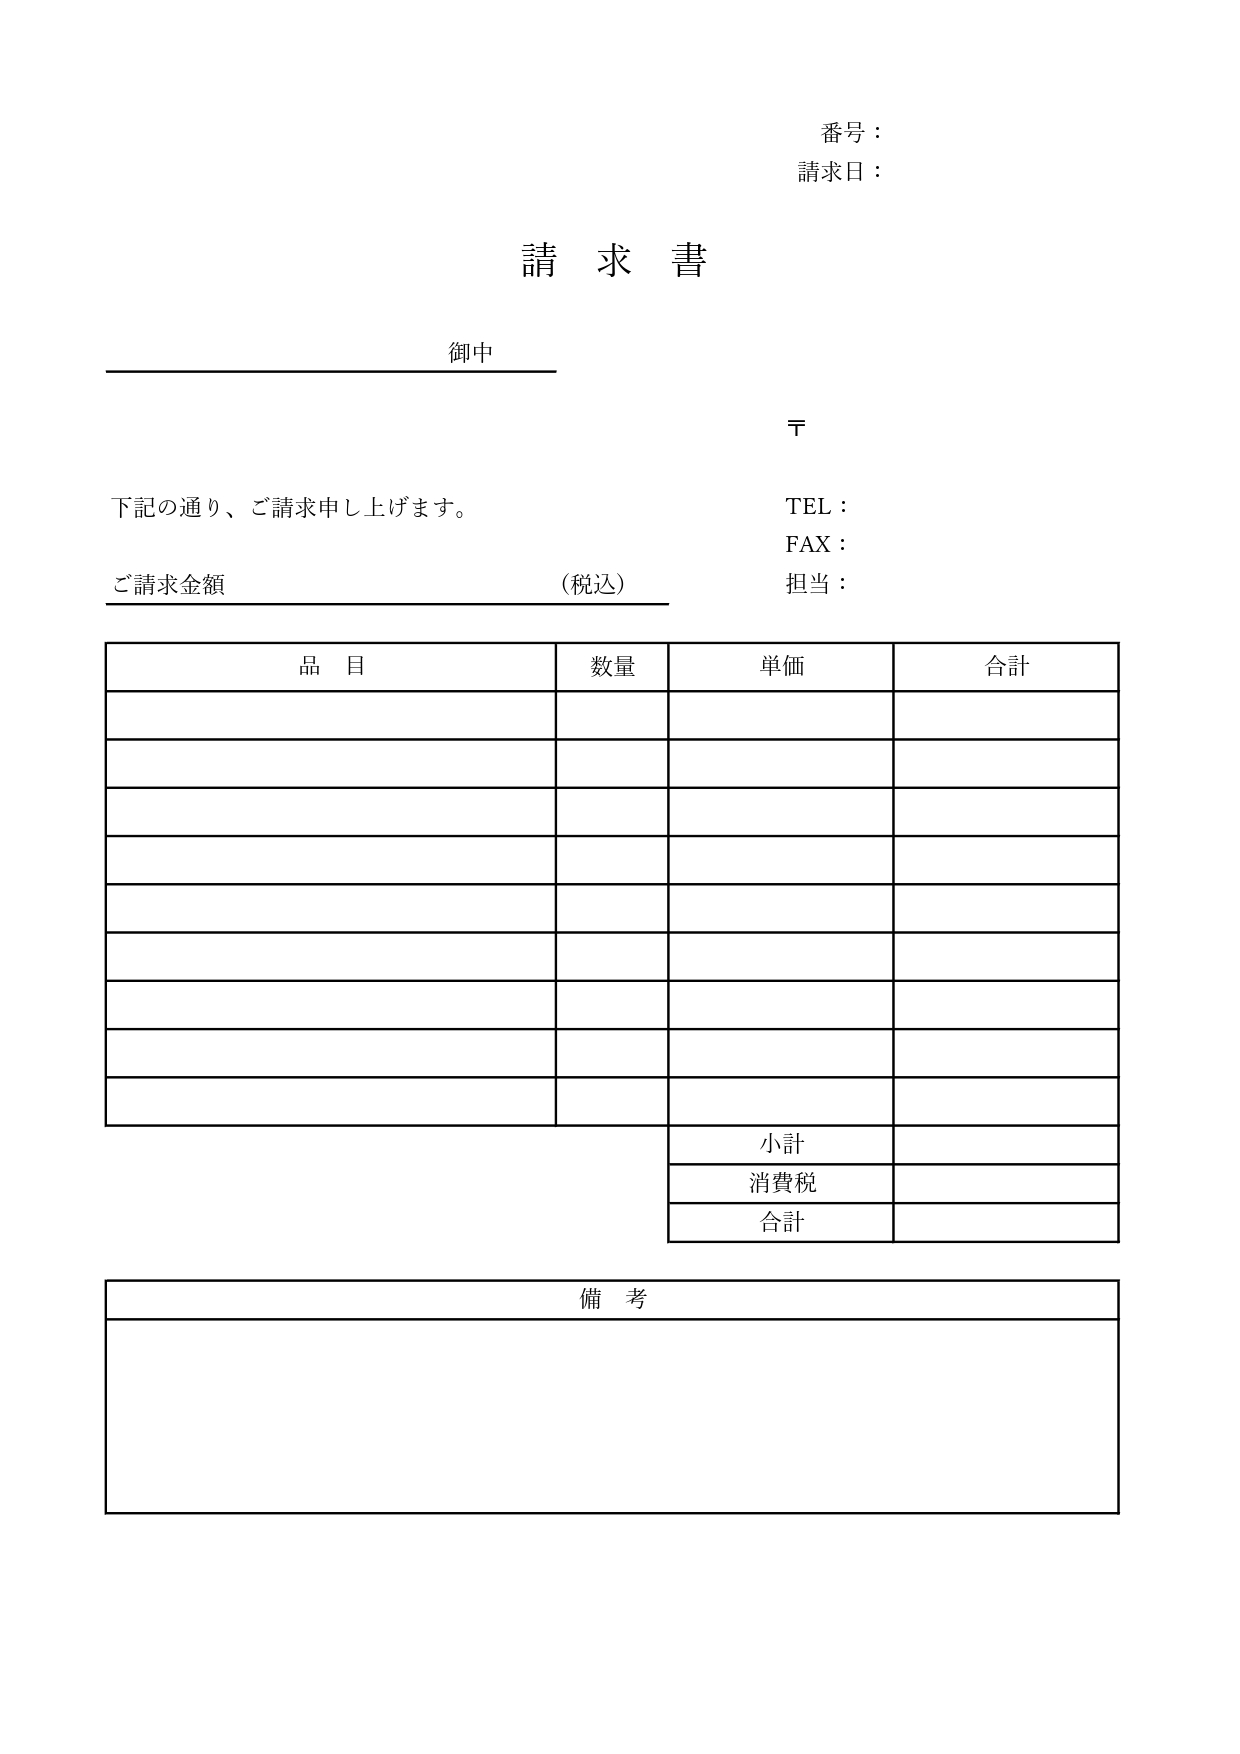
\includegraphics[width=15cm]{image/03-function/original.jpg}
      \caption{元画像}
      \label{fig:original}
  \end{center}
\end{figure}


\section{電子フォーム記入欄取得機能}\label{sec:eform_write_space_obtainment_feature}
電子フォーム記入欄取得機能では、取得対象の記入欄である矩形領域および下線部領域について各領域座標を電子フォーム記入欄として取得する。

電子フォーム記入欄の取得は、以下の手順で行う。

\begin{enumerate}
  \item 矩形領域取得
  \item 下線部領域取得
\end{enumerate}

\subsection{矩形領域取得}\label{subsec:rect_coords_obtainment}
矩形領域取得は、矩形の領域を帳票画像記入欄とみなし、各頂点のxy座標を領域座標として取得する。

図\ref{fig:original}内にある帳票画像記入欄の一部を切り取った画像を、図\ref{fig:rect_original}に示す。
また、図\ref{fig:rect_original}の元画像に対し、矩形の領域座標を取得し、描画した画像を、図\ref{fig:rect_drawing}に示す。
図\ref{fig:rect_drawing}の画像は、JSON形式のファイルでの出力を確認するため、矩形領域座標を参照してランダムなRGBカラーで矩形を描画し、同色で矩形左上隅に番号を表示している。
図\ref{fig:rect_drawing}の矩形に表示する番号は、JSON形式のファイルにある番号と一致する。

\begin{figure}[t]
    \begin{center}
        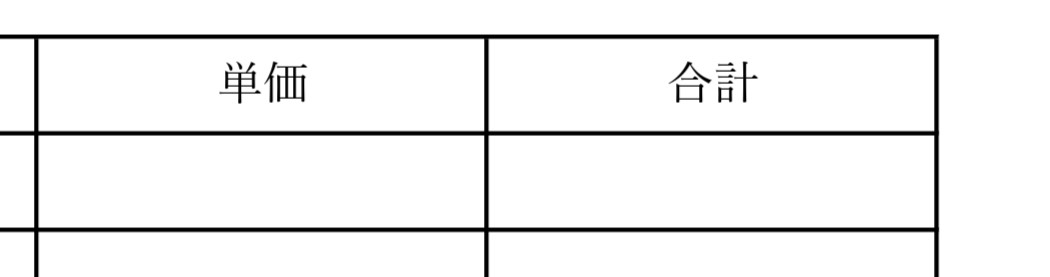
\includegraphics[width=15cm]{image/03-function/rect_original.jpg}
        \caption{帳票画像にある矩形の記入欄}
        \label{fig:rect_original}
    \end{center}
\end{figure}

\begin{figure}[t]
    \begin{center}
        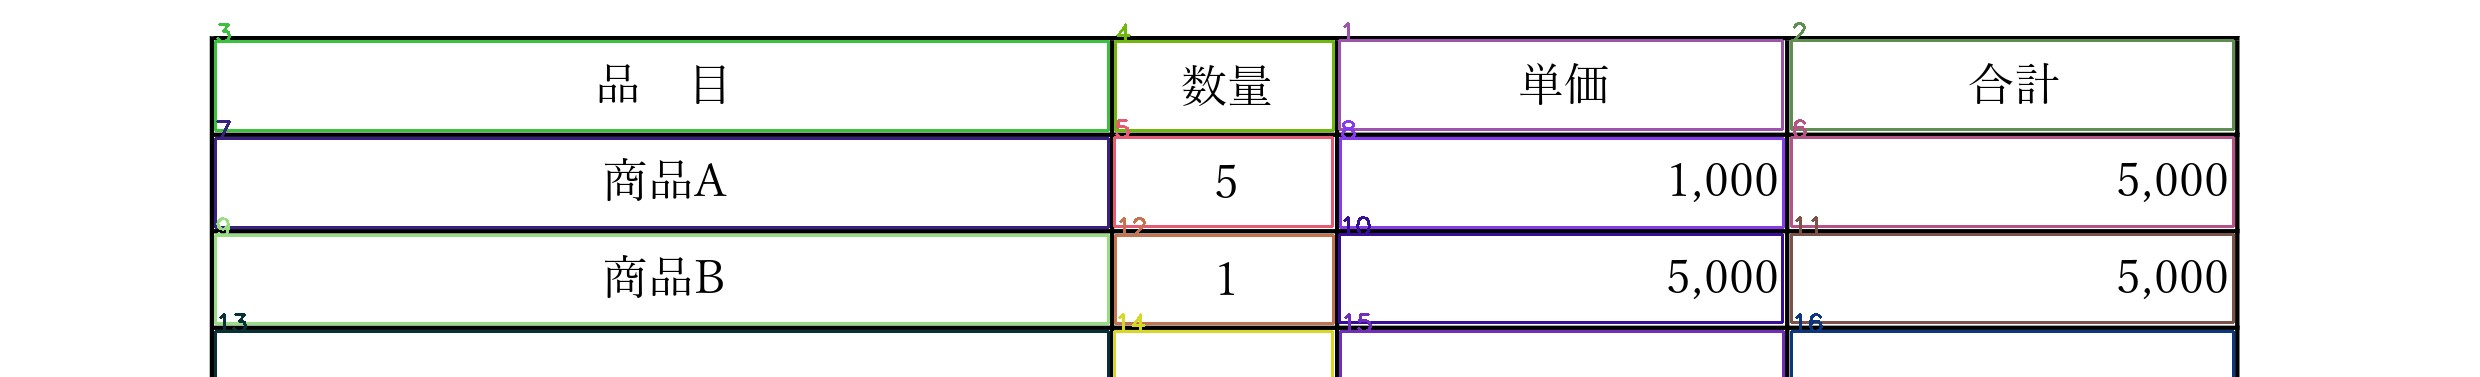
\includegraphics[width=15cm]{image/03-function/rect_drawing.jpg}
        \caption{取得した矩形領域座標の描画}
        \label{fig:rect_drawing}
    \end{center}
\end{figure}



\subsection{下線部領域取得}\label{subsec:underline_coords_obtainment}
下線部領域取得は、水平な直線上の領域を帳票画像記入欄とみなし、両端点のxy座標を領域座標として取得する。

ある帳票画像の一部にある下線部の記入欄を、図\ref{fig:underline_original}に示す。
また、図\ref{fig:underline_original}の画像に対し、下線部の領域座標を取得し、描画した画像を、図\ref{fig:underline_drawing}に示す。
図\ref{fig:underline_drawing}の画像は、JSON形式のファイルでの出力を確認するため、下線部の領域座標を参照して緑色で直線を描画し、同色で直線の左端点上に番号を表示している。
図\ref{fig:underline_drawing}の下線部に表示する番号は、JSON形式のファイルにある番号と一致する。

\begin{figure}[t]
  \begin{center}
      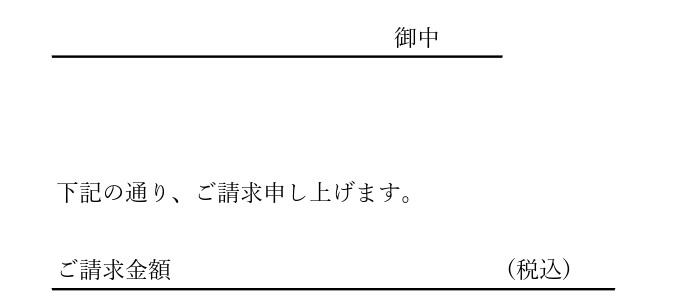
\includegraphics[width=15cm]{image/03-function/underline_original.jpg}
      \caption{帳票画像にある下線部の記入欄}
      \label{fig:underline_original}
  \end{center}
\end{figure}

\begin{figure}[t]
  \begin{center}
      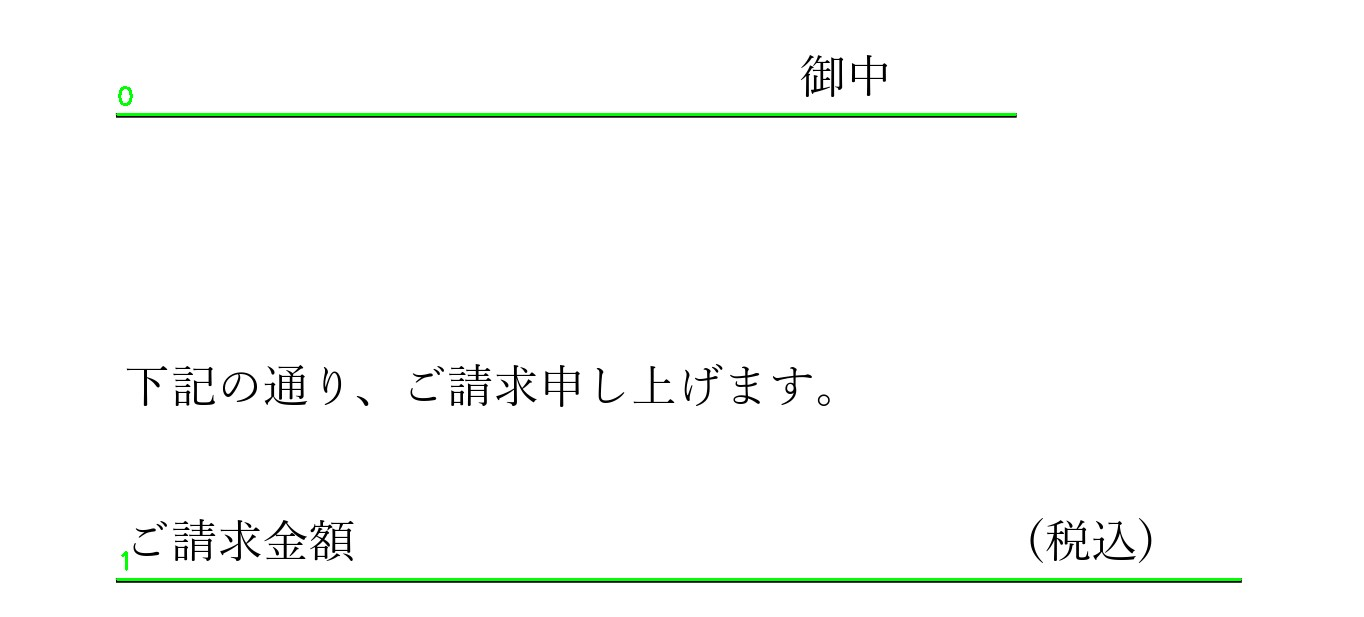
\includegraphics[width=15cm]{image/03-function/underline_drawing.jpg}
      \caption{取得した下線部領域座標の描画}
      \label{fig:underline_drawing}
  \end{center}
\end{figure}



この処理では、確認用出力画像として、領域座標を参照して緑色の直線を描画し、同色で直線の左端点上に番号を表示した画像を出力する。
左端点上に表示する番号は、下線部の全領域座標について、左端点のy座標を昇順にソートしたものに、0から昇順に番号をつける。
左端点のy座標が同じ領域座標が複数存在する場合は、さらに左端点のx座標を昇順にソートしている。
コンソールには、直線の番号と両端点のxy座標を出力する。
コンソールに表示する直線の番号と、確認用出力画像に表示する番号は一致する。


\section{電子フォーム記入欄ラベル付与機能}\label{sec:label_link}
電子フォーム記入欄ラベル付与機能は、\ref{sec:eform_write_space_obtainment_feature}節で電子フォーム記入欄として取得した領域座標に対して、ラベルを付与する。
電子フォーム記入欄にラベルを付与することにより、バリデーションチェックに必要な情報を付与することができる。

本機能は、以下の順で処理を施すことにより、電子フォーム記入欄にラベルを付与する。

\begin{enumerate}
  \item 文字と文字位置の取得
  \item 属性推測
  \item ラベル割付
\end{enumerate}

\subsection{文字と文字位置の取得}\label{subsec:char_and_bbox_obtainment}
入力である帳票画像に対して文字認識を行い、検出した文字と、検出した文字を囲むバウンディングボックスの各頂点の座標をそれぞれ取得文字、文字位置として取得する。
この処理では、確認用出力画像として、文字位置を参照して赤色のバウンディングボックスを描画し、同色でバウンディングボックスの

\subsection{属性推測}\label{subsec:att_prediction}
取得文字に対して、大規模言語モデルによる属性の推測を行う。
以下に、属性の候補を定義する。

\begin{itemize}
	\item 日付(date)
	\item 文字列(string)
	\item 数値(number)
\end{itemize}

以上の属性の候補から、取得文字の属性がいずれに該当するかを推測し、属性として得る。

\subsection{ラベル割付}\label{subsec:label_link}
\ref{sec:eform_write_space_obtainment_feature}節で得た領域座標と、\ref{subsec:char_and_bbox_obtainment}節で得た文字位置、\ref{subsec:att_prediction}節で得た属性を用いる。
文字位置の近傍に存在する領域座標を対象に属性を割り付け、ラベルとして得る。

ラベル割付後、領域座標と、領域座標に対応するラベルを組としたJSON形式のファイルを本提案手法の出力とする。
